\chapter{自动加样系统总体方案的确定}
全自动生化分析仪是一个涉及到多种技术的复杂系统,具有多个功能模块,它的功用要求其具有精度高、可靠性高的特点。研制具有完全自主知识产权的全自动生化分析仪是十分困难的,其中的加样系统会直接影响到系统最后的测定的结果。因此,自动加样系统一直以来都是全自动生化分析仪的关键技术之一,它是一个典型的机电一体化产品,本文的研究对象即为全自动生化仪中的自动加样系统。本部分作为后续章节基础,根据自动加样系统的功用来阐述其基本组成部件,工作原理,硬件组成及控制方法。

\section{自动加样系统的分析}

本自动加样系统主要实现功用为是从样本盘和试剂盘中吸取样本和反应试剂,移送至指定位置,然后利用光学测量机构对二者进行反应结果鉴定;加样动作周期中一个重要的步骤是对加样针进行清洗,以避免试液之间的相互污染。从上述功用可知,自动加样系统一般由进行取样、释放样液(以下简称释样)的加样机构,完成加样功能的机械臂,起到人机交互功能的上位机,控制加样动作的下位机,为防止试剂相互污染的清洗部件以及用来放置盛放待检试剂的小型试管盘。

\section{加样机构的选定}
根据样品加样方式及其原理的不同,加样机构主要有三种结构\supercite{bib3},分别如下:

(1)蠕动泵结构。蠕动泵运用了手指挤压充满液体的软管的原理滚轮替换手指,并在滚轮向前滚动时向前移动液体。通过交替挤压和释放泵的柔性输送软管来泵送流体。就像用手指捏住软管一样,当手指移动时,管内积聚负压,液体流动工作原理图如\ref{fig:2-1}。

\begin{figure}[htbp!]
  \centering
  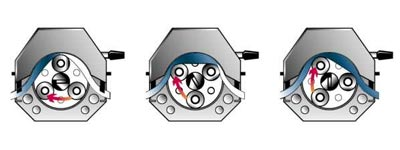
\includegraphics[height=3.5cm]{chap/figure/2-1.jpg}
  \caption{蠕动泵工作原理图}
  \label{fig:2-1}
\end{figure}

蠕动泵的特点明显:一方面,由于运送的材料只接触软管,不接触外界环境,故材料不易受外界环境的污染;其结构决定了蠕动泵的稳定精度好、重复精度高;运送真空度非常高;不需要设置阀门机构,故简化了结构同时又不会出现泄漏现象\supercite{bib4};泵的流道是直通的 没有叶片 阀门等设置因此可用来泵送 易阻塞、含不规则固体颗粒及纤维质物料的流体\supercite{bib4},对运送材料形态要求低;可以输送各种具有磨蚀、腐蚀性,易氧化材料等,运送材料种类广泛。只有软管是需要更换的部件,故更换、维护方便。另一方面,由于蠕动泵使用的软管硬度一定,故其承受压力会受到限制;并且,泵在滚轮交替运作时会产生一个脉冲流,从而导致发生回吸现象,有一定的加样误差。

(2)推入式自动加样结构。推入式自动加样器是以手动加样为原理进行设计的。其动作过程为:从装有样液的试管内吸取一定的试液,移动至加样入口,将试液注入。这种自动加样器设计非常简单,通常只需一根针(上下)移动,样品盘旋转,直到所需的样品瓶位于针下方。使用时,高精度的步进电机带动丝杠配合具导向功能的注射滑块上的传动螺母为动力的传输方式,驱动注射器活塞做往返直线滑动,实现自动精密的定量加样。步进电机在数字脉冲信号响应下,作用于直线轴承实现直线往复运动\supercite{bib5}。此外,注射器的吸入和排出都在步进电机的控制下完成并且采用精密的结构件和合理的驱动方式,此方式可以实现高精度和高准确度,具有良好的稳定性与自动化控制,其结构原理图如\ref{fig:2-2}。

\begin{figure}[htbp!]
  \centering
  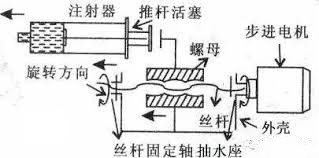
\includegraphics[height=4.8cm]{chap/figure/2-2.jpg}
  \caption{推入式自动加样结构工作原理图}
  \label{fig:2-2}
\end{figure}

(3)六通阀自动加样结构。该结构一般包括两个组成部分:密封垫及固定底座。其大体分为两类:一类是电机驱动的,另一类是用压缩气体驱动的。对于压缩气体驱动结构,利用气动阀内外的压力差,气动阀的一端连接气泵,取样时气动阀内为负压,释放样液时气动阀内为正压。由于采用气动阀,系统要保证良好的气密性,而一旦发生气体泄漏,会对实验分析造成很大的影响,另外气动阀的运动力比电动的会大一些,导致设备噪音大;对于电动结构来说:上部为驱动部分,主要通过程序的执行与否驱动上部。从运动传动角度来看,电动通常属于直接式驱动,气动则属于间接式驱动。

六通阀自动加样结构的加样方法有:部分装液法和完全装液法。采用部分装液法加样时,加样量一般是定量环体积的四分之三,且要保证每次相同的加样体积;采用完全装液法加样时,加样量最少为定量环体积的3至5倍从而保证完全置换样品定量环内残留的溶液以达到所要求的精密度及重现性。为防止缓冲盐和其它残留物质留在加样系统中,每次结束后应冲洗加样器,通常用不含盐的稀释剂、水或不含盐的流动液反复冲洗,再用无纤维纸擦净注射器针头的外侧。由此可知,六通阀自动加样结构对操作人员的加样操作要求高,难以保证加样精度和样液不受外界污染。该结构该结构的工作原理图如\ref{fig:2-3}。

\begin{figure}[htbp!]
  \centering
  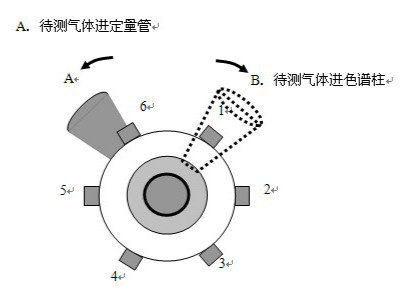
\includegraphics[height=6.5cm]{chap/figure/2-3.jpg}
  \caption{六通阀自动加样结构工作原理图}
  \label{fig:2-3}
\end{figure}

综合比较以上三种加样结构,推入式自动加样结构具有复杂的设计要求,该结构采用丝杠传动且在加样的需求使得步进电机转动方向更换频繁,在此过程中即会出现回程误差,进而造成取样体积出现误差;注射器直接与待检试剂进行接触,不可避免会造成试剂的交叉污染从而造成重大实验损失;此外,该结构零部件更换不方便、难以进行调整以及维护。六通阀自动加样结构的加样阀易于遭受试剂样本中微粒的堵塞和磨损,生命周期短;每次使用前后都要对加样器进行反复的冲洗以避免交叉污染,操作复杂,工作效率低下。此外,六通阀自动加样结构对气密性具有较高的要求,容易受到操作环境变化的影响。而蠕动泵结构操作简单,去离子水和吸入的空气可以有效防止试剂的交叉污染,无加样阀不需要进行密的安全保障;关于运输压力的局限性,我们可以通过增加滚轮的数量降低流量从而降低对软管的压力,使用脉冲抑制器来减少甚至避免液体回吸,脉冲抑制器是一个简单的定位容器,它基于气体可压缩性强于液体可压缩性的工作原理,即脉冲流进入容器、液体上的气袋下陷吸收脉冲进而平缓的流出。当然它的最大缺点是软管易于磨损,但相比于其具有良好的性价比,这是可以接受的。综上所述,本设计的加样结构选用蠕动泵加样结构。

%蠕动泵在工作过程中滚轮会交替挤压软管,当滚轮离开软管%的瞬间会产生回吸现象。当进行加样时回吸现象会严重影响%加样精度,不适用于制造加样精度级高的全自动生化分析仪%。%


















